\chapter{Experimentelle Auswertung}

\section{Teilweise Evaluation}

asdasdasdasdad

\subsection{Abstand Filter}

skdakljdkasdjklasdjaskljdlaksdjladjladjaldjakljdlajdakl

\begin{figure}
\centering
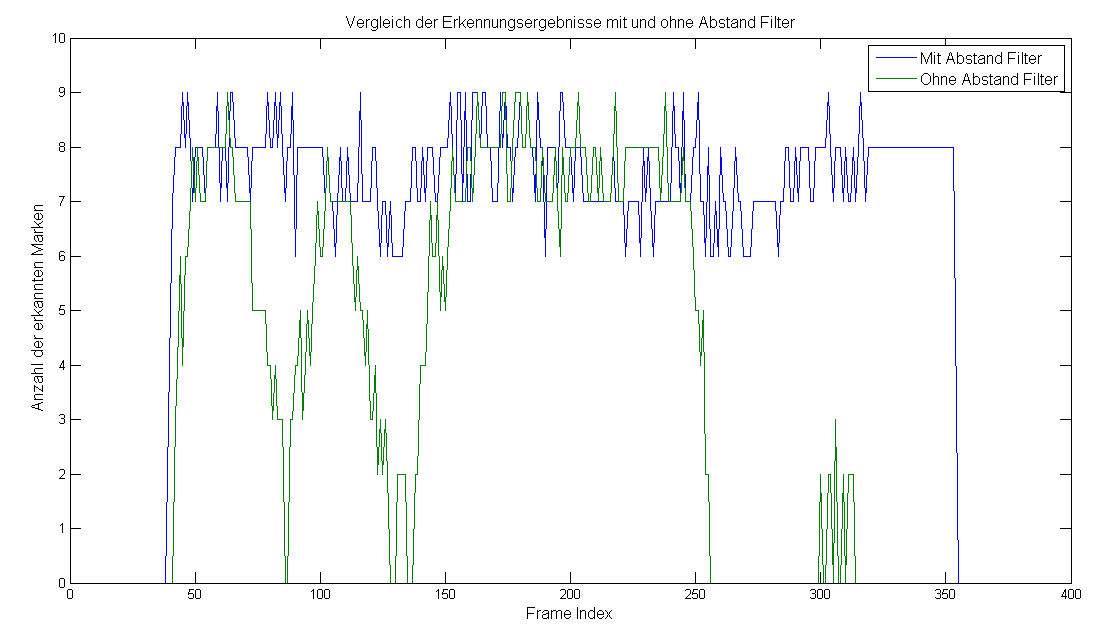
\includegraphics[scale=0.5]{Abbildungen/DF_Empty.png}
\caption{Vergleich der Erkennungsergebnisse mit und ohne Abstand Filter. Die Eingabebilder enthalten nur ein Objekt.}
\label{DFE}
\end{figure}


\begin{figure}
\centering
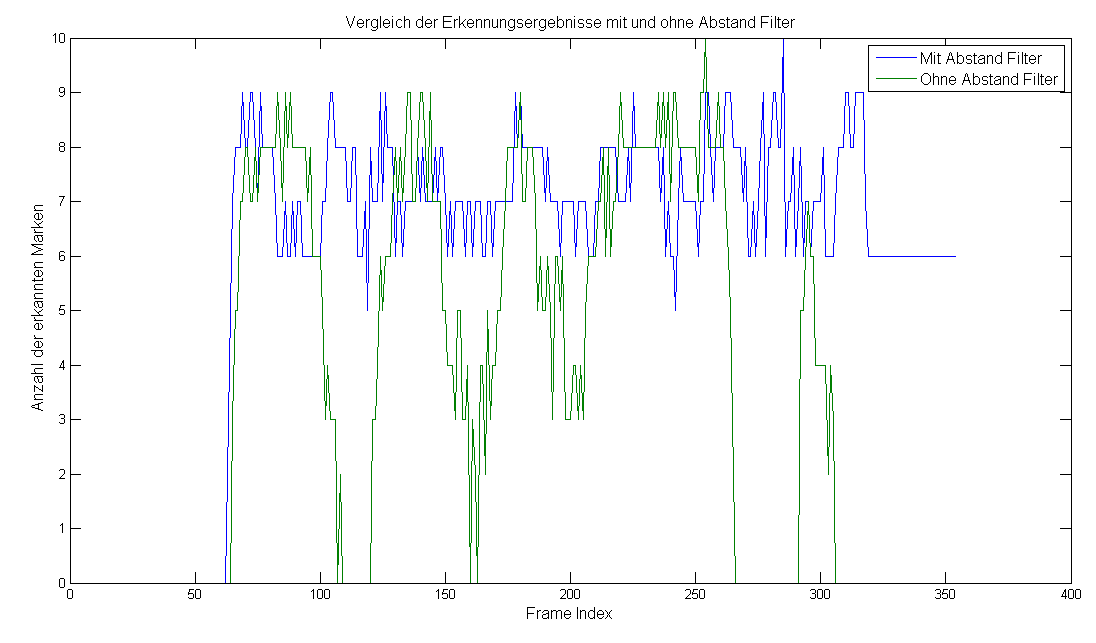
\includegraphics[scale=0.5]{Abbildungen/DF_Full.png}
\caption{Vergleich der Erkennungsergebnisse mit und ohne Abstand Filter. Die Eingabebilder enthalten mehr Objekte.}
\label{DFF}
\end{figure}

\subsection{Helligkeitssteuerung}

\subsection{Verbesserung der Singul�rwertzerlegungsverfahren}

\subsection{Aktualisierung des Strukturgraphen}

\subsection{Teilgraph-Isomorphismus}

\subsection{Bildersteuerung}

\section{Globale Evaluation}